% Hevea - ITILv3 Resumo
% An ITILv3 overview.
%
% Author: José Lopes de Oliveira Jr. <jilo.cc>
%
% LICENSE
% This program is free software: you can redistribute it and/or modify
% it under the terms of the GNU General Public License as published by
% the Free Software Foundation, either version 3 of the License, or
% (at your option) any later version.
%
% This program is distributed in the hope that it will be useful,
% but WITHOUT ANY WARRANTY; without even the implied warranty of
% MERCHANTABILITY or FITNESS FOR A PARTICULAR PURPOSE.  See the
% GNU General Public License for more details.
%
% You should have received a copy of the GNU General Public License
% along with this program.  If not, see <http://www.gnu.org/licenses/>.
%%


%%
% PREAMBLE
%
\documentclass[12px,a4paper,twoside]{book}

% Draft mark
% Comment these lines in final version.
%\usepackage{draftwatermark}
%\SetWatermarkText{RASCUNHO}
%\SetWatermarkScale{4}

% General Purpose Packages
\usepackage{amsfonts}   % To use \times char
\usepackage{fancyhdr}
\usepackage{graphicx}   % For including pictures
\usepackage{lastpage}   % Allows using LastPage

% Encoding and Locale
\usepackage[utf8]{inputenc}     % UTF-8 input encoding
\usepackage[T1]{fontenc}        % Extended font encoding
\usepackage[brazilian]{babel}   % Locale is pt_BR

% PDF Properties
\usepackage[pdftitle={Resumo da ITIL},
            pdfauthor={José Lopes Oliveira Jr.},
            pdfsubject={Resumo das características da ITIL},
            pdfkeywords={itil, it, itg}]{hyperref}

% Document Properties
\title{ITIL\textsuperscript{\textregistered}v3: Resumo}
\author{José Lopes Oliveira Jr.}

% Acronym List
\usepackage[notintoc,portuguese]{nomencl}
\makenomenclature


%%
% MAIN
%
\begin{document}
    % Hevea - ITILv3 Resumo
% An ITILv3 overview.
%
% Author: José Lopes de Oliveira Jr. <jilo.cc>
%
% LICENSE
% This program is free software: you can redistribute it and/or modify
% it under the terms of the GNU General Public License as published by
% the Free Software Foundation, either version 3 of the License, or
% (at your option) any later version.
%
% This program is distributed in the hope that it will be useful,
% but WITHOUT ANY WARRANTY; without even the implied warranty of
% MERCHANTABILITY or FITNESS FOR A PARTICULAR PURPOSE.  See the
% GNU General Public License for more details.
%
% You should have received a copy of the GNU General Public License
% along with this program.  If not, see <http://www.gnu.org/licenses/>.
%%


\fancyhead{}  % clear header
\fancyfoot{}  % clear footer
\fancyhead[RO]{\rightmark}  % section name in upper right
\fancyhead[LE]{\leftmark}  % chapter name in upper left
\fancyfoot[LO,RE]{\thepage}  % numbering in outter border


% Preparing for textinfo content
\pagestyle{empty}
\pagenumbering{roman}

% Hevea - ITILv3 Resumo
% An ITILv3 overview.
%
% Author: José Lopes de Oliveira Jr. <jilo.cc>
%
% LICENSE
% This program is free software: you can redistribute it and/or modify
% it under the terms of the GNU General Public License as published by
% the Free Software Foundation, either version 3 of the License, or
% (at your option) any later version.
%
% This program is distributed in the hope that it will be useful,
% but WITHOUT ANY WARRANTY; without even the implied warranty of
% MERCHANTABILITY or FITNESS FOR A PARTICULAR PURPOSE.  See the
% GNU General Public License for more details.
%
% You should have received a copy of the GNU General Public License
% along with this program.  If not, see <http://www.gnu.org/licenses/>.
%%


\begin{titlepage}
\begin{center}
\vspace*{5cm}
\rule{\linewidth}{.5mm}\\[.4cm]
{\huge \bfseries ITIL\textsuperscript{\textregistered}v3: Resumo}\\[.4cm]
\rule{\linewidth}{.5mm}\\[1.5cm]

\begin{minipage}{.4\linewidth}
    \begin{flushleft}
        \large
        \emph{Autor:}\\
        José Lopes \textsc{Oliveira Jr.}
    \end{flushleft}
\end{minipage}
\begin{minipage}{.4\linewidth}
    \begin{flushright}
        \large
        \emph{Publicação:}\\
        Jiló Inc.
    \end{flushright}
\end{minipage}
\end{center}
\end{titlepage}
  % \include{} can't be nested

% Back cover
\hspace{.1cm}\centerline{
\includegraphics[scale=.7]{img/indiecode}}

% Cataloguing rules
\vspace{3.5cm}
\fbox{
    \begin{minipage}[b][7.5cm][c]{\linewidth}
        Oliveira Júnior, José Lopes\\
        ITIL\textsuperscript{\textregistered}v3: Resumo\\
        1\textordfeminine edição, \pageref{LastPage} páginas --- março de 2012\
        \begin{enumerate}
            \item ITIL\textsuperscript{\textregistered}
            \item Tecnologia da Informação
            \item Governança de TI
        \end{enumerate}
        I. Título\\
        \vfill
        Correções, sugestões ou críticas: \url{http://jilo.cc}\\
    \end{minipage}
}

\vspace{1cm}
\hfill\fbox{
    \begin{minipage}{10cm}
        O trabalho \textbf{ITIL\textsuperscript{\textregistered}v3: Resumo} de
        \href{http://jilo.cc}{José Lopes Oliveira Jr.} foi licenciado com uma
        \href{http://creativecommons.org/licenses/by-sa/3.0/br/}{CC BY-SA 3.0
        Brasil}.
    \end{minipage}
}\hfill

% List of elements
\printnomenclature[3cm]  % acronym [3cm] Explanation
\tableofcontents

% Preparing for the content
\newpage
\pagestyle{fancy}
\pagenumbering{arabic}


    % Include chapters
    % Hevea - ITILv3 Resumo
% An ITILv3 overview.
%
% Author: José Lopes de Oliveira Jr. <jilo.cc>
%
% LICENSE
% This program is free software: you can redistribute it and/or modify
% it under the terms of the GNU General Public License as published by
% the Free Software Foundation, either version 3 of the License, or
% (at your option) any later version.
%
% This program is distributed in the hope that it will be useful,
% but WITHOUT ANY WARRANTY; without even the implied warranty of
% MERCHANTABILITY or FITNESS FOR A PARTICULAR PURPOSE.  See the
% GNU General Public License for more details.
%
% You should have received a copy of the GNU General Public License
% along with this program.  If not, see <http://www.gnu.org/licenses/>.
%%


\chapter{Introdução}
\label{cha:intro}


\begin{figure}
    \centering
    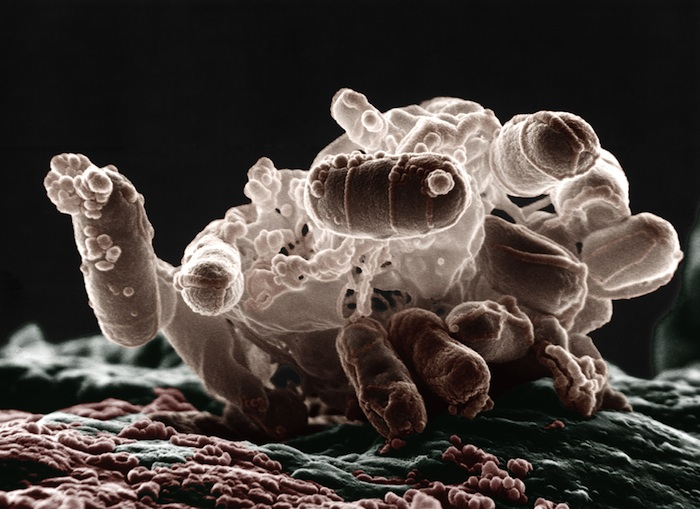
\includegraphics[width=1\textwidth]{img/bacteria_bunch}\\
    {\scriptsize Bunch of Bacteria --- Mirror Lake}
\end{figure}

Ao longo do tempo, a Tecnologia da Informação (TI) passou a obter mais destaque
dentro das organizações. Com isso, o setor passou a ser menos tolerante a
falhas e criou-se a ideia de que ele deveria deixar o posto de simples provedor
de tecnologia, para se tornar um verdadeiro parceiro de negócio para a
organização.
\nomenclature{TI}{Tecnologia da Informação}%

Neste contexto surgiram frameworks de processos e boas práticas. Tais
frameworks buscavam guiar a TI de forma a se organizar melhor e alcançar seu
objetivo. Surgiram também normas para empresas com setores de TI validados
dentro de um determinado padrão, como a ISO 20000.
\nomenclature{ISO}{International Organization for Standardization}%

\section{ITIL\textsuperscript{\textregistered}}
\label{sec:intro:itil}

A ISO 20000 certifica empresas, mas não pessoas. Enquanto norma de
certificação, ela aponta o que se espera que as empresas façam, mas não mostra
em detalhes como fazer isso. A Information Technology Infrastructure Library
(ITIL\textsuperscript{\textregistered}) surge como mais uma solução para
preencher essas lacunas.
\nomenclature{ITIL}{Information Technology Infrastructure Library}%

Desenvolvida pelo Central Computing and Telecommunications Agency\\ (CCTA),
atual Office of Government Commerce (OGC), a
ITIL\textsuperscript{\textregistered} surgiu em 1980 e tornou-se padrão
\emph{de facto} do mercado 10 anos depois. Em 2000, sofreu sua primeira grande
revisão, dando origem à ITIL\textsuperscript{\textregistered}v2 e 7 anos mais
tarde, foi concluída outra revisão que deu origem à
ITIL\textsuperscript{\textregistered}v3.
\nomenclature{CCTA}{Central Computing and Telecommunications Agency}%
\nomenclature{OGC}{Office of Government Commerce}%

Apesar de ser desenvolvida pelo OGC, que é um departamento do governo
britânico, há outras entidades envolvidas com a
ITIL\textsuperscript{\textregistered}. Como o governo britânico não tem
interesse em ganhar dinheiro com este material, ele se limita a gerenciar as
atualizações principais e imprimir os livros. Já que o mercado passou a
considerar importante a certificação de profissionais neste assunto, o OGC
delegou esta tarefa a órgãos não governamentais.

Atualmente, o responsável direto pela certificação de profissionais
ITIL\textsuperscript{\textregistered} é o APM Group (APMG). Mas este órgão
apenas gerencia o esquema de certificação e distribui produtos
ITIL\textsuperscript{\textregistered}. Para desenvolverem uma certificação
profissional para ITIL\textsuperscript{\textregistered}, foram destacados o
Examination Institute for Information Science (EXIN) e o Information Systems
Examinations Board (ISEB).
\nomenclature{APMG}{APM Group Ltd}%
\nomenclature{EXIN}{Examination Institute for Information Service}%
\nomenclature{ISEB}{Information Systems Examinations Board}%

Dessa forma, para se certificar em ITIL\textsuperscript{\textregistered}, o
profissional deve procurar um centro de exames credenciado pelo EXIN ou ISEB.
Ele fará o seu cadastro, marcará e realizará sua prova de certificação.

Cabe ressaltar que existe o Information Technology Service Management Forum
(itSMF), que agrega membros ---empresas e profissionais---, fornecendo um meio
para troca de informações e experiências entre os associados. Normalmente, cada
país tem sua divisão ---capítulo--- do itSMF.
\nomenclature{itSMF}{Information Technology Service Management Forum}%

\section{Certificação}
\label{sec:intro:certi}

A ITIL\textsuperscript{\textregistered}v3 é organizada em 5 livros. O conteúdo
superficial destes livros é cobrado no nível de certificação mais básico:
Foundation. Para conseguir esta certificação, o profissional não precisa
participar de cursos oficiais, nem ter formação na área de TI. Basta estudar o
conteúdo proposto e obter 65\% de acerto na prova de 40 questões ---que deve
ser realizada em até 1 hora, em um dos centros credenciados.

Ao conseguir a aprovação, o profissional receberá um broche, juntamente com o
seu certificado. Este material é enviado diretamente pelo órgão de certificação
a que ele se submeteu ---EXIN ou ISEB. A prova custa em torno de US\$ 150,00 e
é vitalícia. Isso quer dizer que quem se certificou em
ITIL\textsuperscript{\textregistered}v2, não precisa fazer a prova para
ITIL\textsuperscript{\textregistered}v3, pois será um profissional
ITIL\textsuperscript{\textregistered}v2 para sempre.

O nível máximo que se pode chegar em ITIL\textsuperscript{\textregistered}v3 é
o Expert e para isso, precisa-se obter 22 pontos em cursos e provas oficiais.
Para se ter uma ideia, ao obter o ITIL\textsuperscript{\textregistered}
Foundation, o profissional ``ganha'' 2 pontos.

As provas para o ITIL\textsuperscript{\textregistered}v3 Foundation já estão
disponíveis em Português do Brasil e a Prometric é uma das agências mais
flexíveis para se obter essa certificação ---pelo EXIN.

\section{Livros}
\label{sec:intro:livros}

Os 5 livros-base da ITIL\textsuperscript{\textregistered}v3 demostram cada
etapa do ciclo de vida do serviço. Dessa forma, cada livro possui um conjunto
de processos, papéis e funções para realização de cada etapa. Vale lembrar que
a ITIL\textsuperscript{\textregistered} deve ser adequada à realidade de cada
organização. Ela dá ideias do \textbf{quê} pode ser feito, mas não de
\textbf{como} fazer. De fato, a ITIL\textsuperscript{\textregistered} é
bastante flexível e isso se reflete na sua constituição: ela é organizada na
forma de processos, o que a torna aplicável em praticamente qualquer estrutura
de TI. Estes são os os assuntos abordados nos livros da
ITIL\textsuperscript{\textregistered}:
\begin{itemize}
    \item Estratégia de Serviço: descreve como a TI vai se integrar ao negócio,
        deixando de ser reativa e passando a ser proativa.
    \item Desenho de Serviço: projeta o serviço descrito na Estratégia de
        Serviço e define o Acordo de Nível de Serviço (ANS) com o cliente.
    \item Transição de Serviço: coloca o serviço em operação, preparando o
        ambiente para isso.
    \item Operação de Serviço: mantém o serviço funcionando no cotidiano.
    \item Melhoria de Serviço Continuada: avalia o serviço e os processos de
        gerenciamento das fases. Busca melhorar a qualidade, sabendo que um
        serviço não é estável.
\end{itemize}

    % Hevea - ITILv3 Resumo
% An ITILv3 overview.
%
% Author: José Lopes de Oliveira Jr. <jilo.cc>
%
% LICENSE
% This program is free software: you can redistribute it and/or modify
% it under the terms of the GNU General Public License as published by
% the Free Software Foundation, either version 3 of the License, or
% (at your option) any later version.
%
% This program is distributed in the hope that it will be useful,
% but WITHOUT ANY WARRANTY; without even the implied warranty of
% MERCHANTABILITY or FITNESS FOR A PARTICULAR PURPOSE.  See the
% GNU General Public License for more details.
%
% You should have received a copy of the GNU General Public License
% along with this program.  If not, see <http://www.gnu.org/licenses/>.
%%


\chapter{Fundamentos}
\label{cha:fund}


\begin{figure}
    \centering
    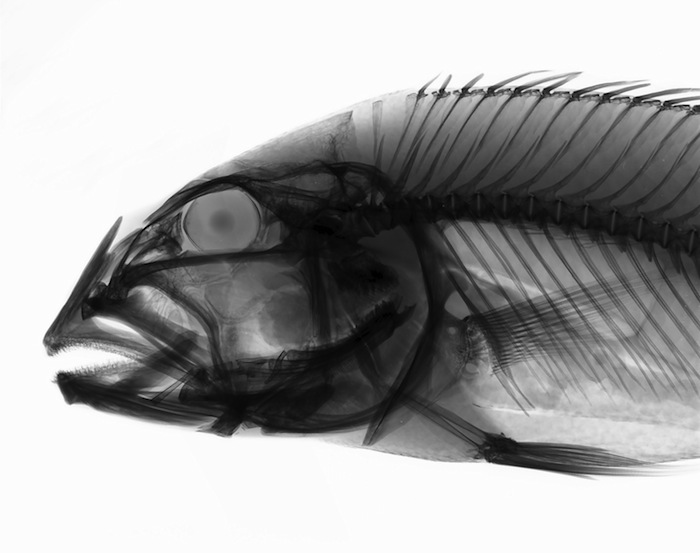
\includegraphics[width=1\textwidth]{img/fish_xray}\\
    {\scriptsize Fish X-Ray --- Arstochromis Christyi}
\end{figure}

Serviço é um meio de entregar valor aos clientes, facilitando os resultados que
eles querem alcançar, sem ter que assumir custos e riscos. Quando se adquire um
carro, por exemplo, o comprador quer que o mesmo se locomova sem ter que se
preocupar com os componentes mecânicos que possibilitam isso.

O Gerenciamento de Serviços de TI (Information Technology Service Management
--- ITSM) é um conjunto de habilidades da organização para fornecer valor ao
cliente em forma de serviços. Quando uma organização passa a depender da TI
para funcionar, esta pode ser encarada como um Ativo Estratégico.
\nomenclature{ITSM}{Information Technology Service Management}%

Ativos de Serviços ---Recursos e Habilidades--- são usados pelo provedor de TI
para entregar um serviço. Recursos são necessários para a produção de um bem ou
realização de um serviço ---e.g., um computador, software, capital financeiro.
Habilidades são a capacidade  da organização de usar os recursos para produzir
valor ---e.g., conhecimento, processos, organização.

Para se criar valor para os serviços é necessário unir Utilidade e Garantia.
Utilidade diz respeito ao que o cliente quer ---e.g., imprimir um documento.
Garantia diz respeito a como o cliente quer receber o serviço ---e.g., como a
impressora é gerenciada para imprimir documentos.


\section{Processos, Funções e Papéis}
\label{sec:funda:proc}

Estes são termos importantíssimos dentro da
ITIL\textsuperscript{\textregistered}, sendo o seu entendimento primordial para
o sucesso da certificação.

Uma organização normalmente é composta por setores. Isso é ruim, pois dificulta
a comunicação e tira o foco dos funcionários ---em vez de pensarem no cliente,
pensam no seu gerente. Processos buscam resolver esses problemas.

\textbf{Processo} é um conjunto estruturado de atividades para produzir um
determinado resultado. Processos não podem existir sozinhos. Alguém precisa
executá-los. Então existem as funções.

\textbf{Função} é um time ou grupo de pessoas e ferramentas usadas para um ou
mais processos e atividades. Como é necessário que todo processo tenha um
proprietário e responsáveis por executá-lo, surgem os papéis.

\textbf{Papel} é um conjunto de responsabilidades e autoridades concedidas a
uma pessoa ou time.

É importante notar que  um papel não é um cargo, assim como um processo não é
um setor dentro de uma empresa. Dessa maneira, uma pessoa pode desempenhar
vários papéis e a implantação dos processos torna-se independente da estrutura
organizacional da empresa.

A ITIL\textsuperscript{\textregistered}v3 é composta por 5 etapas que juntas
têm um total de 24 processos. Cada processo é iniciado por um gatilho e passa
ser controlado e desenvolvido pelas pessoas nas funções específicas dele. Essas
pessoas usam habilidades e recursos para realizar cada atividade que compõe o
processo, gerando a saída do mesmo.

Note que um processo deve ser mensurável e orientado ao cliente. Além disso,
todo processo tem um proprietário, que assegura que o desenvolvimento
transcorra como acordado e documenta tudo isso, para atingir os objetivos
propostos. Já o Proprietário do Serviço, faz o primeiro contato com o cliente e
é responsável pelo serviço como um todo.


\section{Matriz RACI}
\label{sec:funda:raci}

A matriz RACI é usada para definir papéis para execução de um processo. Ela
recebe este nome por ser composta por 4 especificações:
\nomenclature{RACI}{Responsible, Accountable, Consulted, Informed}%
\begin{itemize}
    \item Responsible: os responsáveis pela atividade.
    \item Accountable: prestador de conta da atividade (normalmente é o
        proprietário do processo --- somente uma pessoa pode receber esta
        atribuição dentro de uma atividade).
    \item Consulted: pessoas que serão consultadas na necessidade de
        compartilhamento de uma informação.
    \item Informed: pessoas que devem ser informados durante o progresso.
\end{itemize}


\section{Ciclo de Vida do Serviço}
\label{sec:funda:ciclo}

É composto por fases que levam o nome e são definidas em cada um dos 5 livros
da ITIL\textsuperscript{\textregistered}v3: Estratégia de Serviço, Desenho de
Serviço, Transição de Serviço, Operação de Serviço e Melhoria de Serviço
Continuada.

Cada fase do ciclo de vida recebe como entrada, a saída da anterior e gera
entradas para a próxima. É interessante notar que a Melhoria de Serviço
Continuada, apesar de aparecer por último na sequência, faz parte de todo o
ciclo de vida. Dessa forma, não se chega num ponto para buscar a melhoria do
serviço: ela deve estar presente em todas as fases.

    % Hevea - ITILv3 Resumo
% An ITILv3 overview.
%
% Author: José Lopes de Oliveira Jr. <jilo.cc>
%
% LICENSE
% This program is free software: you can redistribute it and/or modify
% it under the terms of the GNU General Public License as published by
% the Free Software Foundation, either version 3 of the License, or
% (at your option) any later version.
%
% This program is distributed in the hope that it will be useful,
% but WITHOUT ANY WARRANTY; without even the implied warranty of
% MERCHANTABILITY or FITNESS FOR A PARTICULAR PURPOSE.  See the
% GNU General Public License for more details.
%
% You should have received a copy of the GNU General Public License
% along with this program.  If not, see <http://www.gnu.org/licenses/>.
%%


\chapter{Estratégia de Serviço}
\label{cha:estrat}


\begin{figure}
    \centering
    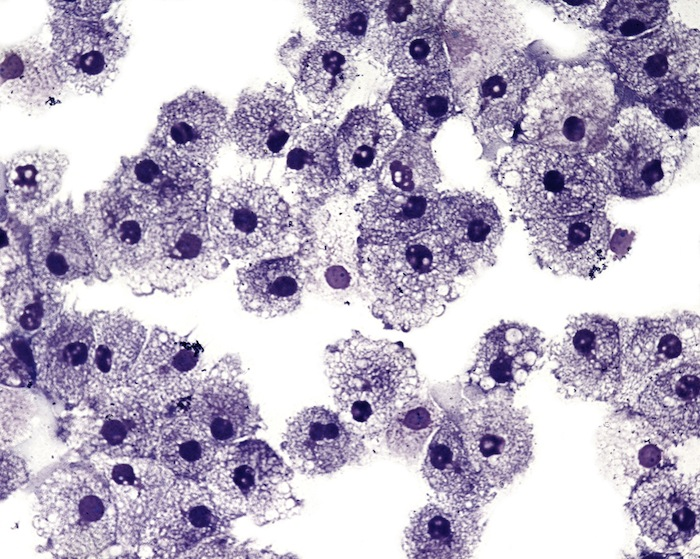
\includegraphics[width=1\textwidth]{img/cell_biology}\\
    {\scriptsize Cell Biology --- The University of New Mexico}
\end{figure}

Nesta fase, todo o planejamento com relação ao serviço será feito, de forma com
que a TI se alinhe ao negócio, tornando-se um ativo estratégico. É preciso
entender que todo serviço de TI tem como propósito sustentar um processo de
negócio.

A fase de Estratégia de Serviço usa uma abordagem multidisciplinar para o
desenvolvimento de serviços. Dessa forma, profissionais de várias áreas dentro
da empresa são envolvidos. O objetivo disso vem da seguinte reflexão: ``O
cliente não compra um serviço ou produto. Ele compra uma solução para resolver
necessidades específicas.''

A TI precisa se alinhar ao negócio para trabalhar de acordo com as necessidades
dos clientes e \emph{stakeholders} (envolvidos no negócio).


\section{4 Ps da Estratégia}
\label{sec:estrat:4ps}

É um conceito desenvolvido no livro Estratégia do Serviço (Mintzberg).
\begin{itemize}
    \item Perspectiva: dá a direção para o provedor de serviço ---missão, visão
        e valores da organização.
	\item Posição: é a imagem que a organização quer passar para os clientes.
	\item Plano: descreve como a organização vai executar a estratégia.
    \item Padrão: é resultado dos 3 Ps anteriores e representa os procedimentos
        da organização, as ações que ela vai tomar.
\end{itemize}


\section{Criação de Valor}
Acontece quando se une os efeitos da Utilidade e da Garantia. É preciso que a
TI crie valor para a organização, para justificar sua existência.


\section{Portfolio de Serviços}
É a representação de todos os serviços de TI e seus estados. É composto por 3
componentes:
\begin{itemize}
    \item Pipeline de Serviços: também conhecido como Funil de Serviços, irá
        conter todos os serviços futuros ---propostos ou em desenvolvimento. É
        a famosa lista de pedidos de aplicações e funcionalidades que os
        usuários enviam. Com o alinhamento da TI ao negócio, quem decide o que
        será implementado é a estratégia da organização.
    \item Catálogo de Serviços: contém os serviços de TI que são oferecidos aos
        clientes e aqueles que foram liberados e entrarão em operação em breve.
    \item Serviços Obsoletos: serviços que estavam em operação e já foram
        aposentados.
\end{itemize}


\section{Catálogo de Serviço}
É como um menu de restaurante e define os serviços acessíveis pelos clientes de
forma mais descritiva que o Portfolio de Serviços. Há 2 tipos:
\begin{itemize}
    \item Catálogo de Serviço do Negócio: está disponível para os clientes, em
        uma linguagem apropriada a eles.
    \item Catálogo de Serviço Técnico: não está visível para o cliente, pois
        contém detalhes técnicos de todos os serviços entregues.
\end{itemize}


\section{Business Case (Plano de Negócio)}
É um documento que possui todos os requisitos de qualidade e custos para que um
serviço opere.


\section{Riscos}
São definidos como um resultado incerto, uma oportunidade positiva ou uma
ameaça. Para gerenciá-los, deve-se fazer um controle das vulnerabilidades,
usando algum framework. Tem 2 etapas distintas:
\begin{itemize}
	\item Análise de Risco: coleta informações sobre a exposição ao risco.
    \item Gerenciamento dos Riscos: gera processos para monitorar e acessar
        informações sobre os riscos, além de processos de tomada de decisão.
\end{itemize}


\section{Modelos de Serviço}
São a forma com que o provedor pretende entregar o serviço ao cliente.


\section{Atividades}
Colocam em prática a estratégia da organização. São elas:
\begin{itemize}
    \item Definir o mercado: entender o cliente e as oportunidades. Classificar
        e visualisar os serviços.
    \item Desenvolver a oferta: definição dos serviços baseados em resultados.
        Portfolio, funil e catálogo de serviço. Utilidade + Garantia: como o
        serviço vai gerar valor para o cliente?
    \item Desenvolver ativos estratégicos: gerenciar o serviço como um ativo
        estratégico para a organização.
    \item Preparar para execução: fazer análise do serviço ---estratégia,
        fatores críticos, competição--- e priorizar investimentos. Matriz SWOT
        ---pontos fortes, fracos, oportunidades e ameaças.
\end{itemize}
\nomenclature{SWOT}{Strengths, Weaknesses, Opportunities, Threats}


\section{Processos}
\subsection{Gerenciamento Financeiro}
As organizações de TI também têm a necessidade de analisar, empacotar, vender e
entregar serviços assim como qualquer empresa. Este processo ajuda na tomada de
decisões ---é preciso saber quanto custa para desenvolver e manter um novo
serviço.

Ajuda também a saber se o serviço gera, de fato, valor para o negócio. É
composto por Orçamento, Contabilidade de TI e Cobrança ---este último, quando
aplicável.

TI é um provedor de serviços e não um provedor de tecnologia.

O Gerente Financeiro será o papel do responsável por este processo.


\subsection{Gerenciamento da Demanda}
Excesso ou falta de capacidade podem gerar perdas para o negócio. Aqui podem
ser definidos ANSs, previsões, planejamento e coordenação com o cliente, para
reduzir a incerteza da demanda ---mas não eliminá-la, pois isso é impossível.
\nomenclature{ANS}{Acordo de Nível de Serviço}

Este processo analisa, rastreia, monitora e documenta os Padrões de Atividade
do Negócio (PAN), que dirão como o cliente usa os serviços e quais os períodos
de pico na utilização deles.
\nomenclature{PAN}{Padrões de Atividade do Negócio}%

O Gerente de Demanda ---papel--- será o responsável por este processo, que,
dentre outras coisas, participará na criação dos ANSs, responderá às mudanças
no PAN e fará o monitoramento da demanda e da capacidade.


\subsection{Gerenciamento do Portfolio de Serviço}
Apenas gerencia os serviços e seus estados, não entrando em detalhes na
documentação de funcionalidades do serviço dentro do Catálogo de Serviço.

Define o portfolio, criando um inventário de serviços e validando os dados.
Analisa o portfolio, definindo quais serviços servem apenas para o negócio que
quais o farão crescer. Aprova o portfolio, autorizando serviços e recursos para
o futuro e eliminando serviços do portfolio atual. Contrata serviços,
comunicando decisões, alocando recursos e fornecendo todo o planejamento para
começar a próxima etapa do ciclo de vida.

O papel criado neste processo é o de Gerente de Produto, que é uma função comum
na área de marketing. Ele é quem vai gerenciar os serviços como produtos e
avaliará as novas oportunidades de mercado, modelos de operação, tecnologia e
necessidades dos clientes.

    % Hevea - ITILv3 Resumo
% An ITILv3 overview.
%
% Author: José Lopes de Oliveira Jr. <jilo.cc>
%
% LICENSE
% This program is free software: you can redistribute it and/or modify
% it under the terms of the GNU General Public License as published by
% the Free Software Foundation, either version 3 of the License, or
% (at your option) any later version.
%
% This program is distributed in the hope that it will be useful,
% but WITHOUT ANY WARRANTY; without even the implied warranty of
% MERCHANTABILITY or FITNESS FOR A PARTICULAR PURPOSE.  See the
% GNU General Public License for more details.
%
% You should have received a copy of the GNU General Public License
% along with this program.  If not, see <http://www.gnu.org/licenses/>.
%%


\chapter{Desenho de Serviço}
\label{cha:design}


\begin{figure}
    \centering
    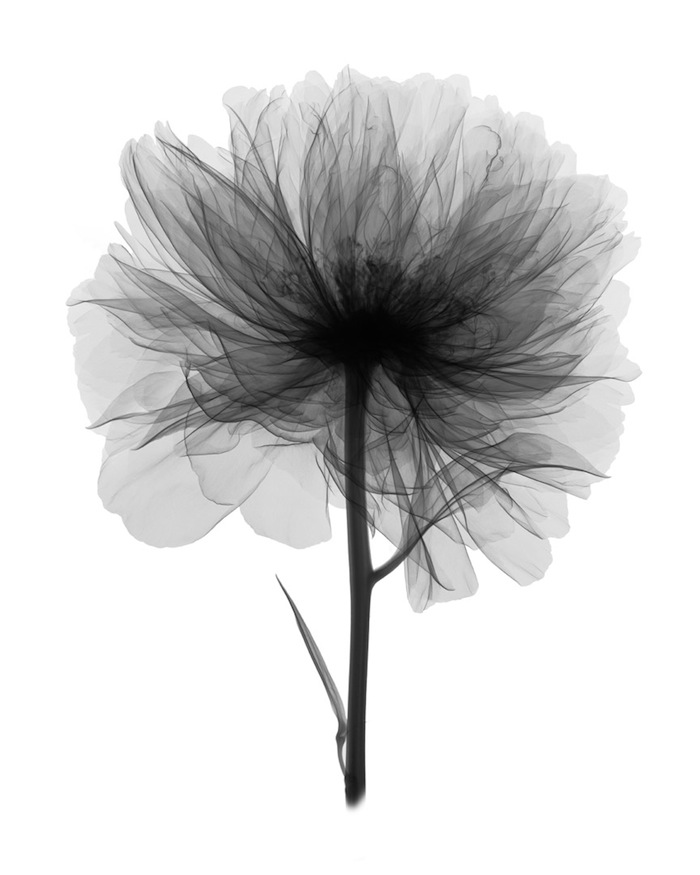
\includegraphics[width=0.5\textwidth]{img/peony}\\
    {\scriptsize Peony --- X-Ray Arts}
\end{figure}

É o desenho de serviços de TI apropriados e invadores, incluindo suas
arquiteturas, processos, políticas e documentações, para suprir requisitos de
negócio atuais e futuros. Desenha serviços que são desenvolvidos dentro de uma
escala de tempo e custo, respeitando os ANSs.


\section{Conceitos}
\label{sec:design:conc}
\begin{itemize}
    \item Provedor de Serviço: é a entidade responsável pela entrega de um
        serviço aos clientes e negócio.
    \item Fornecedor: são os prestadores de serviço externos.
    \item ANS: o Acordo de Nível de Serviço descreve os serviços de TI que o
        provedor deve entregar e os níveis de serviço requeridos. Horário de
        atendimento, tempo de resposta e percentual de disponibilidade são
        algumas da metas que podem ser estabelecidas.
    \item ANO: para que o provedor de serviço consiga cumprir as metas
        estabelecidas nos ANS com o cliente, é necessário que ele estabeleça
        metas internas com suas equipes técnicas. Estas metas internas são
        chamadas de Acordo de Nível Operacional.
    \item Contrato: é relevante que todos os serviços entregues por terceiros
        estejam baseados em um contrato ---também conhecido como Contrato de
        Apoio---, pois ele tem um valor legal entre as partes. Os acordos não
        têm valor legal, são apenas documentos que homologam as metas entre as
        partes.
    \item Pacote de Desenho de Serviço: é uma documentação do projeto para cada
        novo serviço, mudança de grande impacto, remoção de um serviço ou
        mudança em um Pacote de Desenho de Serviço.
    \item Disponibilidade: é a proporção de tempo que um cliente está
        habilitado a acessar, quando requerido, um serviço específico ou a
        habilidade de executar uma função acordada. É mensurada a partir do
        ponto de vista do cliente e registrada no ANS. O tempo/percentual da
        disponibilidade de um serviço deve ser compatível com o tempo de
        serviço acordado.
\end{itemize}
\nomenclature{ANO}{Acordo de Nível Operacional}


\section{Os 4 Ps}
\label{sec:design:4ps}
\begin{itemize}
    \item Pessoas: é importante determinar os papéis das pessoas nos processos.
    \item Processos: devem ser bem definidos.
    \item Produtos: precisam ser determinados, inclusive serviços.
    \item Parceiros: devem ser estabelecidos
\end{itemize}

Os 4 Ps se interrelacionam e representam as competências necessárias que o
provedor de serviços deve ter.


\section{Algumas Opções de Fornecimento de Serviço}
\label{sec:design:ofs}
\begin{itemize}
    \item Insourcing: utiliza recursos internos à organização.
    \item Outsourcing: utiliza recursos externos à organização.
    \item Co-sourcing: combina in e outsourcing.
    \item Multi-sourcing: arranjo para organizações trabalharem em conjunto, as
        atividades são distribuídas por vários fornecedores.
\end{itemize}


\section{Processos}
\label{sec:design:processos}
\subsection{Gerenciamento de Nível de Serviço}
É responsável por garantir entendimento entre as necessidades dos clientes e o
que o provedor de TI deve entregar. Estabelecer acordos ---ANSs--- é uma forma
de gerenciar a expectativa do cliente, pois ele saberá o que poderá exigir do
provedor, que se beneficiará por passar a ter um claro entendimento do que deve
entregar.

Gerente de Nível de Serviço é o papel descrito neste processo e suas atividades
incluem, dentre outras, garantir que as metas de níveis de serviço estão
alinhadas com os ANSs, revisar acordos internos e externos e analisar a
satisfação do cliente.


\subsection{Gerenciamento do Catálogo de Serviço}
Proporciona um único local de informações consistentes sobre todos os serviços
acordados e assegura que o catálogo esteja disponível para quem tem autorização
de acessá-lo. O Catálogo de Serviço está inserido dentro do Portfolio de
Serviço, entretanto, este documento é bem mais estruturado e tem informações
detalhadas dos serviços.

O Gerente de Catálogo de Serviço é responsável por produzir e manter o
catálogo.


\subsection{Gerenciamento de Disponibilidade}
Tem como meta assegurar que os serviços sejam entregues dentro dos níveis
acordados. É completado por 2 níveis relacionados:
\begin{enumerate}
    \item Disponibilidade do Serviço, que envolve todos os aspectos da
        disponibilidade de um serviço; e
    \item Disponibilidade do Componente, que envolve aspectos da
        disponibilidade de um componente do serviço.
\end{enumerate}

A disponibilidade é envolvida por 4 aspectos:

\begin{itemize}
    \item Disponibilidade: habilidade de um serviço, componente ou item de
        configuração executar a função acordada quando requerida;
    \item Confiabilidade: medida de quanto tempo um serviço, componente ou item
        de configuração pode executar a função acordada sem interrupção;
    \item Sustentabilidade: rapidez que um serviço, componente ou item de
        configuração consegue ser restaurado para seu estado normal após uma
        falha; e
    \item Funcionalidade: habilidade de um fornecedor externo em atender os
        termos de seu contrato.
\end{itemize}

O Gerente de Disponibilidade garante que todos os novos serviços são desenhados
para entregar o nível de disponibilidade requerido pelo negócio, dentre outras
funções.


\subsection{Gerenciamento da Segurança da Informação}
Visa controlar a provisão de informações e evitar seu uso não autorizado. Seus
objetivos são compostos por:
\begin{itemize}
    \item Confidencialidade: o acesso à informação será feito de forma correta;
    \item Integridade: a informação será completa e precisa;
    \item Disponibilidade: a informação estará disponível quando requerida; e
    \item Autenticidade: as trocas de informação entre a organização e seus
        parceiros será confiável.
\end{itemize}

Controles de segurança precisam ser estabelecidos para atender aos requisitos
de entidades externas, como Banco Central e Sarbanes Oxley (SOX). A Política de
Segurança da Informação é o resultado deste processo.

Este documento estabelece um conjunto de controles que atendem os objetivos
internos à organização e regulamentos e leis externas. O Gerenciamento da
Segurança da Informação é baseado na ISO/IEC 27001 que estabelece as seguintes
etapas: Controlar, Planejar, Implantar, Avaliar e Manter.

O Gerente de Segurança é quem desenvolve e publica a Política de Segurança da
Informação na organização e garante que ela está sendo usada.


\subsection{Gerenciamento de Fornecedor}
Assegura que os fornecedores e os seus serviços são gerenciados para suportar
as metas dos serviços de TI e os ANSs. Assegura que contratos e acordos com
fornecedores estejam alinhados com as necessidades do negócio e com as metas
dos ANSs e ANOs, em conjunto com o Gerenciamento do Nível de Serviço.

O Banco de Dados de Contratos é um repositório central onde ficam os cadastros
de todos os fornecedores e os contratos relacionados. Dessa forma, os
fornecedores podem ser classificados conforme sua avaliação de risco e impacto:
\begin{itemize}
    \item Estratégicos: envolvem troca de informação confidencial;
    \item Táticos: envolvem atividades comerciais significativas;
    \item Operacionais: fornecem serviços ou produtos de operação; e
    \item Commodity: fornecedores de papel, tinta etc.
\end{itemize}

Cada fornecedor precisa de um tratamento diferenciado conforme sua importância.

Neste processo é definido o papel de Gerente de Fornecedor, que será
responsável por todas as tarefas descritas, catalogando, mantendo, avaliando,
comunicando e negociando contratos com fornecedores.


\subsection{Gerenciamento de Capacidade}
Assegura que a capacidade da infraestrutura de TI esteja alinhada com as
necessidades do negócio. Entende e mantém os níveis de entrega de serviços
resquisitados a um custo aceitável. Está continuamente tentando alcançar a
combinação de custo efetivo com os recursos de TI. É divido em 3 subprocessos:
\begin{itemize}
    \item Gerenciamento da Capacidade do Negócio: focado no longo prazo,
        assegura que os requisitos do negócio sejam levados em consideração;
    \item Gerenciamento da Capacidade de Serviço: assegura que a performance
        dos serviços estejam de acordo com os ANSs; e
    \item Gerenciamento da Capacidade de Componente: mais detalhado e técnico,
        otimiza a utilização dos recursos de hardware e software.
\end{itemize}

O Gerente de Capacidade atua com ponto focal para questões de capacidade e
desempenho, incluindo relatórios de gerenciamento sobre uso, tendências e
previsões.


\subsection{Gerenciamento da Continuidade do Serviço}
Prepara o provedor de serviço para a pior situação possível. Faz parte de um
processo maior, que não é de TI, mas sim da organização como um todo: o
Gerenciamento da Continuidade do Negócio.

Diferentemente do Gerenciamento da Disponibilidade, que foca em obter a melhor
disponibilidade possível para os serviços de TI em operação, o Gerenciamento da
Continuidade do Serviço foca em elaborar um plano de continuidade com
estratégias de recuperação para desastres.

O Gerente de Continuidade do Serviço criará e manterá o processo, assegurando
que ele esteja de acordo com o Gerenciamento de Continuidade do Negócio.
Realizará testes e ajudará na execução da análise de impacto do negócio para
todos os serviços.

    % Hevea - ITILv3 Resumo
% An ITILv3 overview.
%
% Author: José Lopes de Oliveira Jr. <jilo.cc>
%
% LICENSE
% This program is free software: you can redistribute it and/or modify
% it under the terms of the GNU General Public License as published by
% the Free Software Foundation, either version 3 of the License, or
% (at your option) any later version.
%
% This program is distributed in the hope that it will be useful,
% but WITHOUT ANY WARRANTY; without even the implied warranty of
% MERCHANTABILITY or FITNESS FOR A PARTICULAR PURPOSE.  See the
% GNU General Public License for more details.
%
% You should have received a copy of the GNU General Public License
% along with this program.  If not, see <http://www.gnu.org/licenses/>.
%%


\chapter{Transição de Serviço}
\label{cha:trans}


\begin{figure}
    \centering
    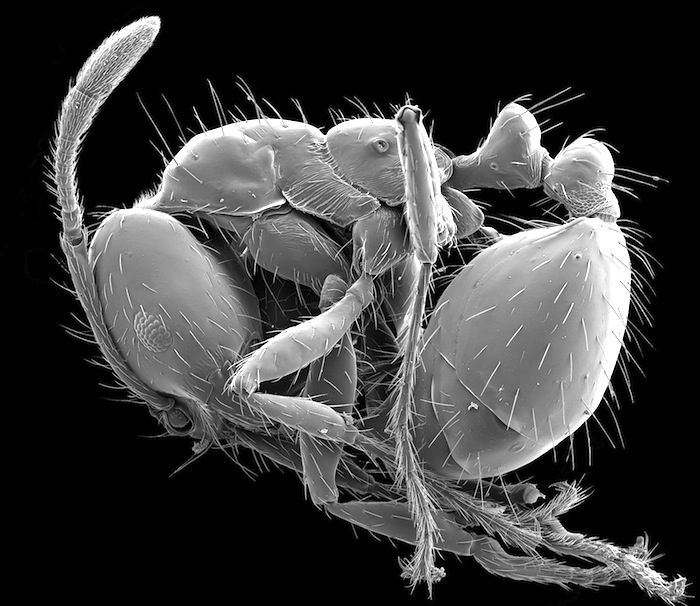
\includegraphics[width=0.7\textwidth]{img/ant_microscope}\\
    {\scriptsize An Army of One --- Arthtopod Image Salon}
\end{figure}

Esta fase ajuda a organização a planejar mudanças nos serviços e implantar
liberações de serviço com sucesso no ambiente de produção. Assegura que haja o
mínimo de impacto no serviços em produção quando uma mudança ou novo serviço
for implantado. Além disso, garante que os requisitos da Estratégia do Serviço
estejam definidos no Pacote de Desenho de Serviço.


\section{Conceitos}
\begin{itemize}
    \item Item de Configuração (IC): é um ativo, componente do serviço ou
        qualquer outro item que está ou estará sob o controle do processo de
        Gerenciamento da Configuração. Exemplos: servidores, aplicativos,
        documentações de processos, Pacote de Desenho de Serviço, Plano de
        Negócio.
    \item Banco de Dados de Gerenciamento da Configuração (BDGC): é um
        repositório de informações onde serão armazenados os registros de ICs.
        Cada IC armazenado no BDGC deve ter um identificador único. Usando
        várias aplicações para esta finalidade, a organização poderá ter vários
        BDGCs.
    \item Sistema de Gerenciamento de Configuração (SGC): armazena todas as
        informações dos ICs dentro de um escopo determinado. Os diversos BDGCs
        que existirem na organização precisam ser integrados para que as
        informações não fiquem duplicadas e desatualizadas.
    \item Sistema de Gerenciamento de Conhecimento de Serviço (SGCS): é formado
        por um conjunto de dados em base central. Os BDGCs alimentam o SGC, que
        fornece informações para o SGCS e elas suportam os processos de tomada
        de decisão. A forma com que as pessoas usam as informações gera o
        conhecimento. Não há como armazenar conhecimento, pois ele está
        relacionado a experiências e habilidades das pessoas.
    \item Biblioteca de Mídia Definitiva (BMD): é uma biblioteca segura na qual
        versões autorizadas definitivas de todas as mídias de ICs são
        armazenadas e protegidas ---está mais relacionada aos meios físicos de
        armazenamento do que o BDGC.
    \item Mudança de Serviço: designa uma mudança em um serviço existente ou
        uma introdução de novo serviço no ambiente de produção.
	\item Tipos de Mudanças:
        \begin{itemize}
            \item Padrão: mudança em um serviço ou infraestrutura que é
                pré-autorizada pelo Gerenciamento de Mudança ---é uma rotina
                definida por um script padrão.
            \item Normal: é levantada por um iniciador que requer uma mudança
                ---precisa ser autorizada antes de executada.
            \item Emergencial: precisa ser implantada rapidamente para resolver
                um incidente, por isso nem sempre pode-se realizar todos os
                testes.
        \end{itemize}

	\item 7 Rs do Gerenciamento de Mudança:
        \begin{enumerate}
            \item Raise (Quem submeteu a mudança?)
            \item Reason (Qual é a razão da mudança?)
            \item Return (Qual é o retorno requerido a partir da mudança?)
            \item Risks (Quais são os riscos envolvidos na mudança?)
            \item Resources (Quais são os recursos necessários para entregar a
                mudança?)
            \item Responsible (Quem é o responsável pela mudança?)
            \item Relationship (Qual é a relação entre esta mudança e outras
                mudanças?).
        \end{enumerate}

    \item Unidade de Liberação: descreve a porção de um serviço ou
        infraestrutura de TI que é normalmente liberada de acordo com a
        política de liberação da organização.
    \item Modelo V de Serviço: serve como uma ferramenta para mapear os
        diferentes níveis de configuração que precisam ser construídos e
        testados. Quanto mais cedo os testes forem feitos, mais cedo as falhas
        serão descobertas, evitando-se o retrabalho.
\end{itemize}
\nomenclature{IC}{Item de Configuração}
\nomenclature{BDGC}{Banco de Dados de Gerenciamento da Configuração}
\nomenclature{SGC}{Sistema de Gerenciamento da Configuração}
\nomenclature{SGCS}{Sistema de Gerenciamento de Conhecimento de Serviço}
\nomenclature{BMD}{Biblioteca de Mídia Definitiva}


\section{Processos}
\label{sec:trans:processos}
\subsection{Gerenciamento de Mudança}
Assegura que mudanças são feitas de forma controlada e são avaliadas,
priorizadas, planejadas, testadas, implantadas e documentadas. Gerenciar
mudanças não é fazer mudanças que não ofereçam riscos, mas tornar os riscos
mapeados e gerenciados. Se a TI for muito ágil para implantar as mudanças, pode
provocar incidentes, interrupções e retrabalhos. Se a TI for demasiadamente
burocrática, pode prejudicar o negócio do cliente. O escopo do Gerenciamento de
Mudança cobre as mudanças desde a base de ativos de serviço e ICs até o
completo ciclo de vida do serviço. Cada organização deve definir as mudanças
que ficarão fora do escopo do seu processo de Gerenciamento de Mudança.

Requisição de Mudança (RDM) é uma requisição formal para mudar um ou mais ICs.
O Comitê Consultivo de Mudanças (CCM) é formado por pessoas que se reúnem para
autorizar a mudança e assistir na sua avaliação e priorização.
\nomenclature{RDM}{Requisição de Mudança}
\nomenclature{CCM}{Comitê Consultivo de Mudanças}

O primeiro passo é registrar uma RDM, então os \emph{stakeholders} revisam a
RDM, verificando se ela está em conformidade. Em seguida, a mudança é analisada
e avaliada ---entram aqui os 7 Rs--- e o CCM ou o Gerente de Mudança determina
se a mudança será implantada. Caso seja, determina-se sua prioridade com base
no impacto e na urgência. A próxima etapa é a coordenação da implantação, onde
o Gerenciamento de Liberação e Implantação coordenará as atividades envolvidas
na construção e criação de liberações. Uma vez implantada, a mudança passará
por uma avaliação para checar se ela cumpriu o seu propósito.

O Gerente de Mudança será o responsável por este processo, atuando desde o
registro da RDM junto ao cliente, até a revisão da mudança e a produção de
relatórios.


\subsection{Gerenciamento da Configuração e de Ativo de Serviço}
É o processo que identifica todos os ICs necessários para entregar os serviços
de TI. Certifica que as informações sobre os ICs nos BDGCs são corretas e
atuais. Alguns conceitos são definidos aqui.
\begin{itemize}
	\item Biblioteca Segura: coleção de ICs.
	\item Armazém Seguro: local onde podem ser armazenados ativos de TI.
    \item Biblioteca de Mídia Definitiva: é a Biblioteca Segura onde versões de
        software autorizadas são armazenadas.
    \item Peças Definitivas: Armazém Seguro onde estão as peças sobressalentes
        de hardware.
    \item Linha de Base de Configuração: configuração aprovada de um serviço,
        produto ou infraestrutura.
	\item Instantâneo (Snapshot): cópia do estado atual de um IC ou ambiente.
\end{itemize}

Vários papéis são definidos aqui. Gerente de Ativos de Serviço, Gerente de
Configuração, Analista de Configuração, Bibliotecário de Configuração,
Administrador de Ferramentas SGC.


\subsection{Gerenciamento de Liberação e Implantação}
Faz o controle de versões e controla as instalações de software, hardware e
outros componentes de infraestrutura, do ambiente de desenvolvimento ao
ambiente de testes e depois para o ambiente de produção.Vai assegurar que haja
o mínimo impacto não precedente nos serviços de produção e na organização de
operações e suporte.

Unidade de Liberação é a parte do serviço ou infraestrutura que está incluída
na liberação de acordo com as diretrizes de liberação da organização. A forma
de distrubuição pode ser:
\begin{itemize}
    \item Big Bang: implanta o serviço novo ou alterado para todos os usuários
        ao mesmo tempo;
	\item Fase: é feita para parte dos usuários;
    \item Empurrada: o componente de serviço é implantado à partir da área
        central para usuários em locais remotos;
	\item Puxada: o sistema do usuário é responsável por buscar a atualização; e
    \item Automatizada ou Manual: liberações maiores podem ser automatizadas e
        menores podem ser feitas manualmente.
\end{itemize}

Um Pacote de Liberação pode ser a única Unidade de Liberação ou uma coleção
delas. Este processo consiste basicamente das seguintes atividades:
\begin{itemize}
	\item Planejamento
	\item Preparação para Construção
	\item Teste e Implantação
	\item Construção e Teste
	\item Teste de Serviço e Pilotos
	\item Planejamento para Implantação
	\item Transferência
	\item Implantação e Retirada
	\item Verificação da Implantação
	\item Suporte para o Período de Funcionamento Experimental
\end{itemize}

Os papéis definidos aqui são: Gerente de Liberação e Implantação, Gerente de
Empacotamento e Construção de Liberação, Equipe de Implantação.

    % Hevea - ITILv3 Resumo
% An ITILv3 overview.
%
% Author: José Lopes de Oliveira Jr. <jilo.cc>
%
% LICENSE
% This program is free software: you can redistribute it and/or modify
% it under the terms of the GNU General Public License as published by
% the Free Software Foundation, either version 3 of the License, or
% (at your option) any later version.
%
% This program is distributed in the hope that it will be useful,
% but WITHOUT ANY WARRANTY; without even the implied warranty of
% MERCHANTABILITY or FITNESS FOR A PARTICULAR PURPOSE.  See the
% GNU General Public License for more details.
%
% You should have received a copy of the GNU General Public License
% along with this program.  If not, see <http://www.gnu.org/licenses/>.
%%


\chapter{Operação de Serviço}
\label{cha:opera}


\begin{figure}
    \centering
    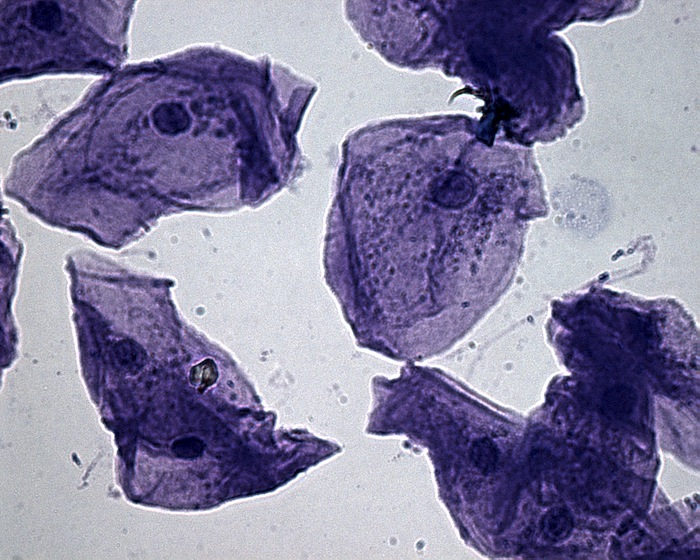
\includegraphics[width=1\textwidth]{img/cheek_cells}\\
    {\scriptsize Cheeck Cells --- 7th Grade Life Science Classroom Blog}
\end{figure}

Introduz, explica e detalha atividades de entrega e controle para alcançar a
excelência operacional de um serviço. É uma fase mais prolongada do ciclo de
vida, pois o serviço deverá ser mantido em bom estado operacional até que perca
sua utilidade e seja aposentado. O propósito desta fase é coordenar e realizar
as atividades e processos requeridos para gerenciar serviços em níveis
acordados com usuários e clientes.


\section{Conceitos}
\label{sec:opera:conceitos}
\begin{itemize}
    \item Requisição de Serviço: é um pedido por uma mudança ou para acessar um
        serviço de TI.
    \item Evento: notificação criada por um serviço, IC ou ferramenta de
        monitoramento causada pelo desvio de desempenho da infraestrutura ou de
        entrega do serviço.
    \item Alerta: aviso ou advertência sobre uma meta, mudança ou falha que
        ocorreu.
    \item Incidente: interrupção inesperada ou redução na qualidade de um
        serviço de TI.
    \item Problema: causa de um ou mais incidentes.
    \item Solução de Contorno: meio temporário de resolver questões ou
        dificuldades.
    \item Erro Conhecido: problema que tem a causa raíz documentada e uma
        Solução de Contorno identificada.
	\item Base de Erros Conhecidos: local onde se registram Erros Conhecidos.
    \item Impacto, Urgência e Prioridade: É importante avaliar o impacto e a
        urgência de incidentes, problemas ou mudanças nos processos de negócio,
        para determinar suas prioridades. Para o impacto deve-se considerar
        quantas pessoas ou sistemas serão prejudicados. Já a urgência determina
        a velocidade com que o incidente precisa ser resolvido.
\end{itemize}


\section{Princípios}
\label{sec:opera:principios}
\begin{itemize}
    \item Visão Interna do Negócio $\times$ Visão Externa do Negócio: ter
        somente a visão interna, pode levar a focar em sistemas pouco
        importantes ao negócio. Ter só a visão externa, pode levar o pessoal de
        TI a prometer o que não pode cumprir.
    \item Estabilidade $\times$ Agilidade: se a TI pensa apenas na
        estabilidade, ela se torna lenta para se adaptar às necessidades do
        negócio. Se ela é muito ágil, não faz um bom planejamento das mudanças
        e perde estabilidade.
    \item Qualidade do Serviço $\times$ Custo do Serviço: a TI precisa fazer um
        uso ótimo dos recursos.
    \item Reativa $\times$ Pró-ativa: uma TI reativa só age com uma pressão
        externa. Uma TI pró-ativa está sempre buscando oportunidades de
        melhorias ---o que pode levar à perda do foco na necessidade real do
        negócio.
\end{itemize}

A lição que se tira destas comparações é que todos estes aspectos precisam ser
balanceados pelo pessoal de TI. Somente assim será possível prover serviços que
gerem valor ao negócio e ao cliente, de  forma eficiente e eficaz.


\section{Processos}
\label{sec:opera:processos}
\subsection{Gerenciamento de Incidente}
Lida com todos os incidentes ---falhas e dúvidas. A meta deste processo é
restaurar a operação normal do serviço o mais rápido possível e minimizar os
impactos adversos nas operações do negócio. Inclui qualquer evento que
interrompa ou que possa interromper um serviço. Faz uso de alguns conceitos:
\begin{itemize}
	\item Limites de Tempo: acorda os limites de tempo de acordo com os ANSs;
    \item Modelos de Incidente: determinam os passos necessários para executar
        o processo corretamente; e
    \item Incidentes Graves: precisam ser resolvidos com urgência, com a
        utilização de um procedimento específico.
\end{itemize}

Neste processo, além do Gerente de Incidente, há as responsabilidades das
equipes de suporte, que poderão ser agrupadas em vários níveis, cada um mais
especializado que o outro. Assim, caso um nível não consiga diagnosticar o
incidente, ele o repassa para o nível imediatamente acima, mais especializado.


\subsection{Gerenciamento de Evento}
Um evento é qualquer ocorrência detectável ou discernível, que seja
significativa para a gestão da infraestrutura de TI ou para a entrega do
serviço de TI e avaliação do impacto que um desvio pode causar aos serviços.

O Gerenciamento de Evento objetiva proporcionar e fornecer entradas para muitos
processos e atividades da Operação de Serviço. Pode ser aplicado para qualquer
aspecto do Gerenciamento de Serviço que precise ser controlado e que pode ser
automatizado.

Não é necessário possuir o papel de Gerente de Evento, pois suas atividades são
delegadas às funções de TI, como a Central de Serviço.


\subsection{Cumprimento de Requisição}
O termo “cumprimento e requisição” é usado como uma descrição genérica para
muitos tipos de variáveis de demandas colocadas sobre o departamento de TI por
seus usuários. Consiste das seguintes atividades:
\begin{itemize}
	\item Seleção de Menu;
	\item Autorização Financeira;
	\item Cumprimento; e
	\item Conclusão.
\end{itemize}

A propriedade do Cumprimento de Requisição fica com a Central de Serviço, que
monitora, escala, despacha e frequentemente preenche as requisições dos
usuários.


\subsection{Gerenciamento de Problemas}
Tem a intenção de encontrar erros conhecidos na infraestrutura de TI. Os
problemas são a causa de um ou mais incidentes. Um incidente nunca vira
problema: sempre haverá 2 registros separados, um para cada processo.

Neste processo há o envolvimento de 2 papéis: Gerente de Problema e Grupos de
Resolução de Problemas.


\subsection{Gerenciamento de Acesso}
Concede ao usuário o direito de usar um serviço e nega acessos de usuários não
autorizados. É composto de alguns conceitos básicos:
\begin{itemize}
    \item Acesso: é o nível que estende a funcionalidade ou dados que um
        usuário pode usar;
    \item Identidade: informação única que distingue um indivíduo, verifica o
        estado;
	\item Direitos: configurações atuais que permitem o acesso dos usuários;
    \item Serviços dos Grupos de Serviço: é o acesso a um conjunto de serviços
        ou grupos de usuários, mas não o acesso separado aos serviços; e
    \item Serviços de Diretório: refere-se a uma ferramenta que permite
        gerenciar acessos e direitos.
\end{itemize}

Este processo é composto das seguintes atividades: Verificação da Legitimidade
das Requisições, Fornecimento dos Direitos, Monitoramento do Estado de
Identidade ---Mudança de Papéis---, Registro e Monitoramento do Acesso, Remoção
e Limitação de Direitos.

O Gerenciamento de Acesso é uma sobreposição do Gerenciamento de Segurança e do
Gerenciamento de Disponibilidade.


\section{Funções}
\subsection{Central de Serviços}
É uma unidade funcional que está envolvida em vários eventos de serviço. Deve
funcionar como um ponto único de contato para os usuários no dia a dia. Há 4
tipos de Central de Serviços:
\begin{itemize}
    \item Local: é criada para atender necessidades locais de cada unidade de
        negócio;
    \item Centralizada: centraliza todas as solicitações de suporte em um único
        local;
    \item Virtual: suporte espalhado por diversos países – sempre que o usuário
        fizer uma chamada, dependendo do horário, ele será atendido por alguém
        em uma posição geográfica diferente; e
    \item Siga o Sol: é a combinação de centrais que estão dispersas
        geograficamente, fornecendo suporte 24 horas/dia a um custo
        relativamente baixo.
\end{itemize}

A equipe de suporte deverá ter as seguintes qualificações, no mínimo:
Habilidades interpessoais, Entendimento dos serviços e Conhecimento técnico.

Os seguintes papéis figuram nesta função: Gerente de Central de Serviços,
Supervisor de Central de Serviços e Analista de Suporte.


\subsection{Gerenciamento Técnico}
É a função responsável por fornecer habilidades técnicas para o suporte de
serviços de TI e para o Gerenciamento da Infraestrutura de TI. Em pequenas
organizações, pode estar em 1 departamento e em grandes organizações, pode
estar distribuído por vários departamentos.


\subsection{Gerenciamento de Aplicação}
É responsável por gerenciar aplicativos durante seu ciclo de vida. Sua função é
realizada por qualquer departamento, grupo ou equipe envolvida na gestão e
suporte de aplicativos operacionais. Uma das decisões-chave à qual ele
contribui é a de comprar um aplicativo ou criá-lo ---que é discutido no Desenho
de serviço, Capítulo \ref{cha:design}. Esta função também pode ser distribuída
em grupos. O Gerenciamento de Aplicação não é responsável pelo desenvolvimento
do software ---é responsável pela manutenção de aplicações.


\subsection{Gerenciamento de Operações de TI}
É a função responsável pela gestão contínua e manutenção de uma infraestrutura
de TI de uma organização, para assegurar a entrega do ANS ao negócio. Consiste
de 2 sub-funções: Controle de Operações de TI e Gerenciamento das Instalações.

    % Hevea - ITILv3 Resumo
% An ITILv3 overview.
%
% Author: José Lopes de Oliveira Jr. <jilo.cc>
%
% LICENSE
% This program is free software: you can redistribute it and/or modify
% it under the terms of the GNU General Public License as published by
% the Free Software Foundation, either version 3 of the License, or
% (at your option) any later version.
%
% This program is distributed in the hope that it will be useful,
% but WITHOUT ANY WARRANTY; without even the implied warranty of
% MERCHANTABILITY or FITNESS FOR A PARTICULAR PURPOSE.  See the
% GNU General Public License for more details.
%
% You should have received a copy of the GNU General Public License
% along with this program.  If not, see <http://www.gnu.org/licenses/>.
%%


\chapter{Melhoria de Serviço Continuada}
\label{cha:melhoria}


\begin{figure}
    \centering
    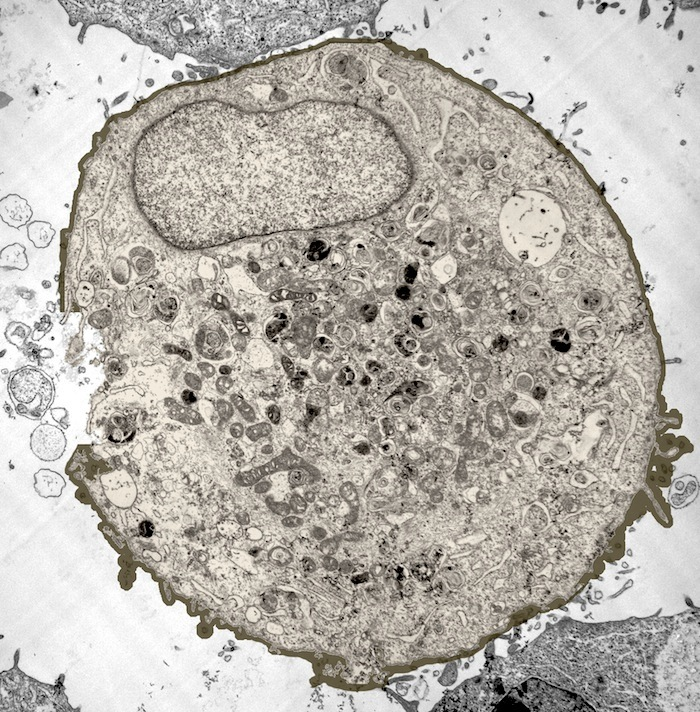
\includegraphics[width=0.7\textwidth]{img/prostate_cancer}\\
    {\scriptsize Prostate Cancer --- Georgia Tech}
\end{figure}

Tem por objetivo proporcionar um guia prático para aumentar a eficiência,
maximizar a efetividade e otimizar o custo dos processos subjacentes ao
Gerenciamento de Serviço de TI e seus processos subjacentes em 3 níveis dentro
da organização: o bom funcionamento do Gerenciamento de Serviço de TI como um
todo; o contínuo alinhamento do Portfolio de Serviços de TI com as necessidades
atuais e futuras do negócio; e a maturidade do processo de TI requerida para
dar suporte aos processos do negócio em um modelo de ciclo de vida de serviço
contínuo.

É importante salientar que esta fase do ciclo de vida não pode ser vista como
uma fase separada. As atividades de melhoria continuada devem ser executadas em
todo o ciclo de vida.


\section{Melhoria de Serviço Continuada no Modelo do Ciclo de Vida do Serviço}
\label{sec:enhan:melhoria}
Cada fase do ciclo de vida gera saídas que servem como entradas para a próxima
fase. A Melhoria de Serviço Continuada faz melhorias em cada fase e no ciclo de
vida como um todo. Ela faz com que o ciclo de vida esteja completamente
integrado.


\section{Mensuração e Melhoria}
\label{sec:enhan:mensura}
É importante ter em mente as seguintes definições:
\begin{quote}
\emph{Não se pode gerenciar o que não se pode controlar.\\
Não se pode controlar o que não se pode medir.\\
Não se pode medir o que não se pode definir.}
\end{quote}

Dessa forma, serviços e processos precisam ser implantados com metas e
objetivos claros e mensuração bem definida.


\section{Ciclo para Implantação da Melhoria de Serviço Continuada}
\label{sec:enhan:ciclo}
Um  serviço é criado por um número de atividades que são agrupadas em
processos. A qualidade dessas atividades e processos determina a qualidade do
serviço. A Melhoria de Serviço Continuada utiliza o ciclo PDCA (Plan, Do,
Check, Act) para aperfeiçoar continuamente a qualidade dos serviços e também a
própria implantação da Melhoria de Serviço Continuada.
\nomenclature{PDCA}{Plan, Do, Check, Act}

Na fase Planejar ---Plan--- são determinados escopo, requisitos que devem ser
atendidos, metas e pontos de ação. Na fase Executar ---Do--- é realizada a
implantação da Melhoria de Serviço Serviço Continuada. Na fase Verificar
---Check--- é realizada a monitoração, mensuração e avaliação. Na fase Agir
---Act--- vem o ajuste para a Melhoria de Serviço Continuada, introduzindo
aperfeiçoamentos para ela.


\section{Modelo de Melhoria de Serviço Continuada}
\label{sec:enhan:modelo}
A ITIL\textsuperscript{\textregistered} recomenda uma abordagem estruturada
para ajudar no aperfeiçoamento, que é o Modelo de Melhoria de Serviço
Continuada. Este ciclo tem 6 fases.
\begin{enumerate}
    \item Determinar a visão: a TI precisa saber quais são as metas do negócio
        e formar uma visão para ajustar a estratégia de TI ao negócio.
	\item Identificar onde se está agora: saber qual a situação atual.
    \item Identificar onde se quer chegar: determinar prioridades baseadas na
        visão do cliente.
    \item Saber como se chega lá: faz-se um plano detalhado de aperfeiçoamento
        do serviço.
    \item Verificar se os objetivos foram alcançados: utilizar a mensuração da
        qualidade para medir os resultados.
	\item Manteneção da qualidade: o ciclo deve ser repetido continuamente.
\end{enumerate}

Processos e serviços precisam ser medidos para:
\begin{itemize}
    \item validar as decisões da estratégia, dirigir as atividades e alcançar
        as metas;
    \item justificar a implantação de mudanças corretivas e para saber em que
        momento devem ser feitas mudanças ou ações corretivas;
    \item ajudar na medição ---a ITIL\textsuperscript{\textregistered}
        recomenda 3 tipos de métricas: Métricas de Serviço, Métricas de
        Processo e Métricas de Tecnologia.
\end{itemize}


\section{Processos}
\label{sec:enhan:processos}
\subsection{7 Passos do Processo de Melhoria}
\begin{enumerate}
	\item Definir o que deve ser medido.
	\item Definir o que se precisa medir.
	\item Coletar dados.
	\item Processar dados.
	\item Analisar dados.
	\item Apresentar e usar a informação.
	\item Implantar ação corretiva.
\end{enumerate}

Este processo envolve os papéis de Gerente de Melhoria de Serviço Continuada,
Gerente de Serviço, Analista de Relatório, Proprietário do Processo de
Gerenciamento do Conhecimento, Proprietários de Processos.

Como são muitos papéis, recomenda-se a utilização de uma matriz RACI para
melhor definir as atividades de cada pessoa.


\subsection{Elaboração de Relatórios}
É responsável pela geração e fornecimento de relatórios sobre os resultados
alcançados e o desenvolvimento nos níveis de serviço. As atividades deste
processo são: Coletar dados, Processar os dados e aplicar para a organização,
Publicar a informação e Ajustar o relatório para o negócio.

\end{document}
